

%% AP Physics MC Questions Archive
%%----------------------------------------

%% Ampere's Law
%%----------------------------------------
\element{ap}{
\begin{question}{amperes-law-q01}
    The magnetic field inside a solenoid of length $l$ is $B$.
    A second solenoid has twice as many turns as the first one and is the same length.
    Both solenoids have the same current passing through them.
    What is the magnetic field inside the second solenoid?
    \begin{multicols}{3}
    \begin{choices}
        \wrongchoice{$\dfrac{B}{4}$}
        \wrongchoice{$\dfrac{B}{2}$}
        \wrongchoice{$B$}
      \correctchoice{$2B$}
        \wrongchoice{$4B$}
    \end{choices}
    \end{multicols}
\end{question}
}

\element{ap}{
\begin{question}{amperes-law-q02}
    What is the magnetic field due to a wire of infinite length carrying a current $I$,
        a distance $a$ away from the wire?
    \begin{multicols}{3}
    \begin{choices}
      \correctchoice{$\dfrac{\mu_0 I}{2\pi}$}
        \wrongchoice{$\dfrac{\mu_0 I}{4\pi}$}
        \wrongchoice{$\mu_0 I$}
        \wrongchoice{$2\pi \mu_0 I$}
        \wrongchoice{$4\pi \mu_0 I$}
    \end{choices}
    \end{multicols}
\end{question}
}

\element{ap}{
\begin{question}{amperes-law-q03}
    What is the magnetic field due to a circular loop of wire carrying a current $I$ and having a radius $R$ at the center of the loop?
    \begin{multicols}{3}
    \begin{choices}
        \wrongchoice{$\dfrac{\mu_0 I}{4\pi R}$}
        \wrongchoice{$\dfrac{\mu_0 I}{4R}$}
        \wrongchoice{$\dfrac{\mu_0 I}{2\pi R}$}
      \correctchoice{$\dfrac{\mu_0 I}{2R}$}
        \wrongchoice{$2\pi \mu_0 IR$}
    \end{choices}
    \end{multicols}
\end{question}
}

\element{ap}{
\begin{question}{amperes-law-q04}
    The Biot-Savart Law is used to:
    \begin{choices}
        \wrongchoice{determine the electric field created by individual point charges}
        \wrongchoice{determine the electric field created by an electric current}
        \wrongchoice{determine the magnetic field created by individual point charges}
      \correctchoice{determine the magnetic field created by an electric current}
        \wrongchoice{determine the force field created by an electric current}
    \end{choices}
\end{question}
}

\element{ap}{
\begin{question}{amperes-law-q05}
    What is the magnitude of the magnetic force on a semicircle of wire of radius $r$ carrying a current $I$ in the plane of the page due to a uniform magnetic field $B$ pointing out of the page?
    \begin{multicols}{3}
    \begin{choices}
        \wrongchoice{$\dfrac{rIB}{2}$}
        \wrongchoice{$rIB$}
      \correctchoice{$2rIB$}
        \wrongchoice{$4rIB$}
        \wrongchoice{$6rIB$}
    \end{choices}
    \end{multicols}
\end{question}
}

\element{ap}{
\begin{question}{amperes-law-q06}
    The below diagram shows a current carrying wire.
    \begin{center}
    \begin{tikzpicture}
        %% Wire
        \draw[thick,-latex] (3,0) -- (0,0);
        \draw[thick,-latex] (0,0) -- (-3,0);
        %% Current
        \node[anchor=north west] at (0,0) {$I$};
        %% Points P
        \draw[fill] (0,-2) circle (2pt) node[anchor=west] {$P$};
        %% distance d
        \draw (-0.5,0) -- (-0.5,-2) node[pos=0.5,anchor=center,fill=white] {$d$};
        \draw (-0.75,-2) -- (-0.25,-2);
    \end{tikzpicture}
    \end{center}
    What is the magnitude and direction of the magnetic field at point $P$ due to the segment of wire above carrying current $I$?
    \begin{choices}
        \wrongchoice{$\dfrac{\mu_0 I}{2\pi d}$ out of the page}
      \correctchoice{$\dfrac{\mu_0 I}{2\pi d}$ into the page}
        \wrongchoice{$\dfrac{\mu_0 I}{4\pi d}$ out of the page}
        \wrongchoice{$\dfrac{\mu_0 I}{4\pi d}$ into the page}
        \wrongchoice{$\dfrac{\mu_0 I}{d}$ out of the page}
    \end{choices}
\end{question}
}

\element{ap}{
\begin{question}{amperes-law-q07}
    What is the magnitude and direction of the magnetic field at point $P$ due to the segment of wire carrying current $I$?
    \begin{center}
    \begin{tikzpicture}[scale=0.66]
        %% Wire
        \draw[thick,-latex] (-4,0) -- (-2,0) node[anchor=south east] {$I$};
        \draw[thick] (-2,0) -- (0,0);
        \draw[thick,-latex] (0,0) -- (0,-2);
        \draw[thick] (0,-2) -- (0,-4);
        %% 90 degree
        \draw (-0.25,0) -- (-0.25,-0.25) -- (0,-0.25);
        %% point P
        \draw[dashed] (0,0) -- (2,0) node[pos=0.5,anchor=south] {$d$};
        \draw[fill] (2,0) circle (2pt) node[anchor=south west] {$P$};
    \end{tikzpicture}
    \end{center}
    \begin{choices}
        \wrongchoice{$\dfrac{\mu_0 I}{2\pi d}$ out of the page}
        \wrongchoice{$\dfrac{\mu_0 I}{2\pi d}$ into the page}
      \correctchoice{$\dfrac{\mu_0 I}{4\pi d}$ out of the page}
        \wrongchoice{$\dfrac{\mu_0 I}{4\pi d}$ into the page}
        \wrongchoice{$\dfrac{\mu_0 I}{d}$ out of the page}
    \end{choices}
\end{question}
}

\element{ap}{
\begin{question}{amperes-law-q08}
    What is the magnetic field at point $P$ due to the segment of wire $AB$ carrying current $I$?
    \begin{center}
    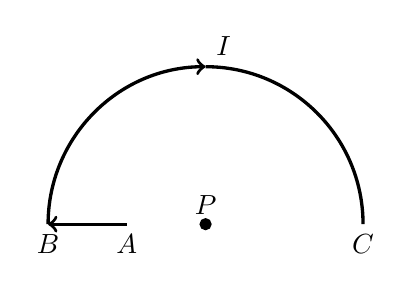
\begin{tikzpicture}
        %% Top Loop
        \draw[very thick,->] (-2,0) arc (180:90:2) node[anchor=south west] {$I$};
        \draw[very thick] (0,2) arc (90:0:2) node[anchor=north] {$C$};
        %% Bottom Straight
        \draw[very thick,->] (-1,0) -- (-2,0)
            node[pos=0,anchor=north] {$A$}
            node[pos=1,anchor=north] {$B$};
        %% Point P
        \draw[fill] (0,0) circle (2pt) node[anchor=south] {$P$};
    \end{tikzpicture}
    \end{center}
    \begin{multicols}{3}
    \begin{choices}
      \correctchoice{zero}
        \wrongchoice{$2\mu_0 Ir$}
        \wrongchoice{$\dfrac{\mu_0 I}{r}$}
        \wrongchoice{$\dfrac{\mu_0 I}{2r}$}
        \wrongchoice{$\dfrac{\mu_0 I}{4r}$}
    \end{choices}
    \end{multicols}
\end{question}
}

\element{ap}{
\begin{questionmult}{amperes-law-q09}
    Which segments of the wire affect the magnetic field at point $P$ for the below wire?
    \begin{center}
    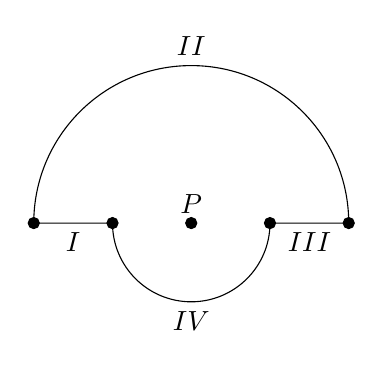
\begin{tikzpicture}
        %% Wire
        \draw (-1,0) -- (-2,0) arc (180:0:2) -- (1,0) arc(360:180:1) -- cycle;
        %% Points
        \draw[fill] (-2,0) circle (2pt);
        \draw[fill] (-1,0) circle (2pt);
        \draw[fill] (0,0) circle (2pt) node[anchor=south] {$P$};
        \draw[fill] (2,0) circle (2pt);
        \draw[fill] (1,0) circle (2pt);
        %% Labels
        \node[anchor=south] at (0,2) {$II$};
        \node[anchor=north] at (-1.5,0) {$I$};
        \node[anchor=north] at (+1.5,0) {$III$};
        \node[anchor=north] at (0,-1) {$IV$};
    \end{tikzpicture}
    \end{center}
    \begin{multicols}{4}
    \begin{choices}
        \wrongchoice{I}
      \correctchoice{II}
        \wrongchoice{III}
      \correctchoice{IV}
        %\wrongchoice{I and III}
        %\correctchoice{II and IV}
        %\wrongchoice{I, II and III}
        %\wrongchoice{II, III and IV}
        %\wrongchoice{I, II, III and IV}
    \end{choices}
    \end{multicols}
\end{questionmult}
}

\element{ap}{
\begin{question}{amperes-law-q10}
    The magnetic field inside a solenoid is $B$.
    A second solenoid has the same number of turns as the first one and is the same length,
        but its radius is twice the size of the radius of the first one.
    Both solenoids have the same current passing through them.
    What is the magnetic field inside the second solenoid?
    \begin{multicols}{3}
    \begin{choices}
        \wrongchoice{$\dfrac{B}{4}$}
        \wrongchoice{$\dfrac{B}{2}$}
      \correctchoice{$B$}
        \wrongchoice{$2B$}
        \wrongchoice{$4B$}
    \end{choices}
    \end{multicols}
\end{question}
}

\element{ap}{
\begin{question}{amperes-law-q11}
    A tightly-wound solenoid has a length of \SI{50}{\centi\meter} and contains a total of 200 turns.
    If it carries a current of \SI{3}{\ampere},
        what is the magnetic field inside the solenoid?
    \begin{multicols}{3}
    \begin{choices}
        %% Added units
        \wrongchoice{$100 \mu_0\,\si{\tesla}$}
        \wrongchoice{$300 \mu_0\,\si{\tesla}$}
        \wrongchoice{$600 \mu_0\,\si{\tesla}$}
      \correctchoice{$1200 \mu_0\,\si{\tesla}$}
        \wrongchoice{$2400 \mu_0\,\si{\tesla}$}
    \end{choices}
    \end{multicols}
\end{question}
}

\element{ap}{
\begin{question}{amperes-law-q12}
    What law is used to calculate the magnetic field inside a toroid?
    \begin{multicols}{2}
    \begin{choices}
        \wrongchoice{Gauss’s law}
      \correctchoice{Ampere's law}
        \wrongchoice{Lenz’s law}
        \wrongchoice{Faraday’s law }
        \wrongchoice{The Biot-Savart law}
    \end{choices}
    \end{multicols}
\end{question}
}

\element{ap}{
\begin{question}{amperes-law-q13}
    An infinitely large current-carrying sheet lies on the $xy$-plane carrying current in the $y$-direction.
    Which of the following is false about the magnetic field that it creates?
    \begin{choices}
        \wrongchoice{The magnetic field depends on the current density in the sheet.}
        \wrongchoice{The magnetic field can be calculated using Ampere’s law.}
      \correctchoice{The magnetic field depends on the distance away from the plane.}
        \wrongchoice{The magnetic field is in the positive x-direction.}
        \wrongchoice{None of the provided}
    \end{choices}
\end{question}
}

\element{ap}{
\begin{question}{amperes-law-q14}
    What is the magnetic field of a very long solenoid with $n$ turns per length and carrying a current $I$?
    \begin{multicols}{3}
    \begin{choices}
        \wrongchoice{$\mu_0 I$}
        \wrongchoice{$2 \mu_0 nI$}
      \correctchoice{$\mu_0 nI$}
        \wrongchoice{$\dfrac{\mu_0 nI}{2}$}
        \wrongchoice{$\dfrac{\mu_0 n}{I}$}
    \end{choices}
    \end{multicols}
\end{question}
}

\element{ap}{
\begin{question}{amperes-law-q15}
    All of the following contribute to the magnetic field outside of an ideal solenoid except?
    \begin{multicols}{2}
    \begin{choices}
        \wrongchoice{physical constants}
        \wrongchoice{length}
        \wrongchoice{number of turns}
        \wrongchoice{current}
      \correctchoice{radius}
    \end{choices}
    \end{multicols}
\end{question}
}

\element{ap}{
\begin{question}{amperes-law-q16}
    Which of the following is not used when applying Ampere's law?
    \begin{multicols}{2}
    \begin{choices}
        \wrongchoice{a line integral}
        \wrongchoice{a dot product}
        \wrongchoice{a length differential}
        \wrongchoice{magnetic field}
      \correctchoice{a surface integral}
    \end{choices}
    \end{multicols}
\end{question}
}

\element{ap}{
\begin{question}{amperes-law-q17}
    What is the magnetic field due to an infinite sheet of charge having current density $\Phi$?
    \begin{multicols}{3}
    \begin{choices}
        %% NOTE: why I?
        \wrongchoice{$\dfrac{\mu_0 I}{2}$}
        \wrongchoice{$\dfrac{\mu_0 I}{2}$}
      \correctchoice{$\dfrac{\mu_0 \Phi}{2}$}
        \wrongchoice{$\mu_0 I$}
        \wrongchoice{$\mu_0 Ø$}
    \end{choices}
    \end{multicols}
\end{question}
}

\element{ap}{
\begin{question}{amperes-law-q18}
    Two wires carry current in the same direction.
    The wires are \SI{10}{\centi\meter} apart.
    \begin{center}
    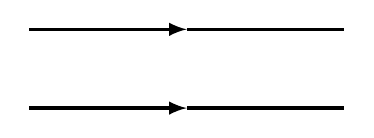
\begin{tikzpicture}
        %% Top wire
        \draw[very thick,-latex] (-2,0) -- (0,0);
        \draw[very thick] (0,0) -- (2,0);
        %% bottom wire
        \draw[very thick,-latex] (-2,-1) -- (0,-1);
        \draw[very thick] (0,-1) -- (2,-1);
    \end{tikzpicture}
    \end{center}
    The upper wire carries a current of \SI{6}{\ampere} and the lower wire carries a current of \SI{4}{\ampere}.
    Where is the magnetic field equal to zero?
    \begin{choices}
        \wrongchoice{\SI{4}{\centi\meter} below the bottom wire}
        \wrongchoice{\SI{6}{\centi\meter} below the bottom wire}
        \wrongchoice{\SI{6}{\centi\meter} above the upper wire }
      \correctchoice{\SI{6}{\centi\meter} below the upper wire}
        \wrongchoice{\SI{6}{\centi\meter} above the bottom wire}
    \end{choices}
\end{question}
}

\element{ap}{
\begin{question}{amperes-law-q19}
    Two wires carry current in opposite directions.
    The wires are \SI{10}{\centi\meter} apart.
    \begin{center}
    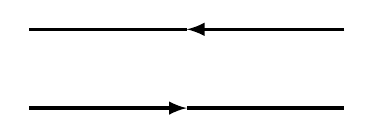
\begin{tikzpicture}
        %% Top wire
        \draw[very thick,-latex] (2,0) -- (0,0);
        \draw[very thick] (0,0) -- (-2,0);
        %% bottom wire
        \draw[very thick,-latex] (-2,-1) -- (0,-1);
        \draw[very thick] (0,-1) -- (2,-1);
    \end{tikzpicture}
    \end{center}
    The upper wire carries a current of \SI{6}{\ampere} and the lower wire carries a current of \SI{4}{\ampere}.
    Where is the magnetic field equal to zero?
    \begin{choices}
        \wrongchoice{\SI{30}{\centi\meter} above the upper wire}
      \correctchoice{\SI{30}{\centi\meter} below the upper wire}
        \wrongchoice{\SI{30}{\centi\meter} above the lower wire}
        \wrongchoice{\SI{30}{\centi\meter} below the lower wire}
        \wrongchoice{None of the provided}
    \end{choices}
\end{question}
}

\element{ap}{
\begin{question}{amperes-law-q20}
    Which of the following laws can be used to calculate the magnetic field from an electric current distribution?
    \begin{choices}
        \wrongchoice{Gauss' Law}
        \wrongchoice{Conservation of Charge}
      \correctchoice{Biot-Sarvart Law}
        \wrongchoice{Faraday's Law}
        \wrongchoice{Gauss's Law for Magnetism}
    \end{choices}
\end{question}
}


\endinput


